% 12 variables in here:
% u_1 = 0.0, h_1 = 10.0, U_1 = 0.0, H_1 = 10.0, u_2 = -1.0, h_2 = 10.0, U_2 = 0.0, H_2 = 10.0, u_3 = 0.0, h_3 = 10.0, U_3 = 0.0, H_3 = 10.0
\begin{figure}[h!t]
\centering
  \subfigure[Height for points $p_1^L$ and $p_3^L$ (same for $p_1^R$ and $p_3^R$ respectively).] {
    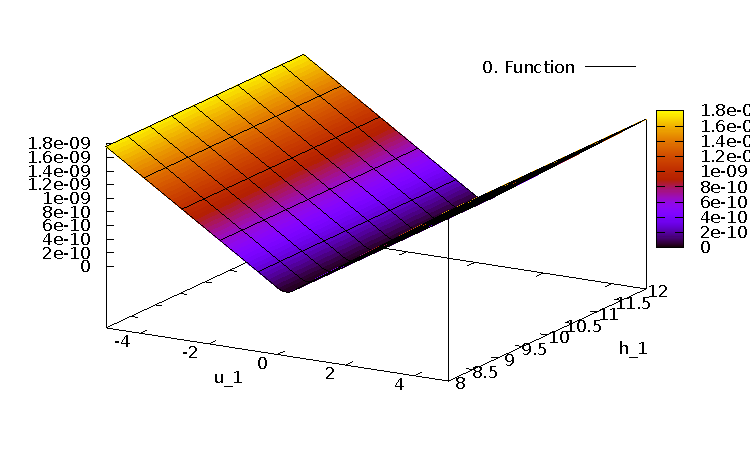
\includegraphics[scale=\zoomfactor]{{{3_punkte_2_impuls_verringert/x_y_0.0_10.0_-1.0_10.0_0.0_10.0_0.0_10.0_0.0_10.0f0}}}  
    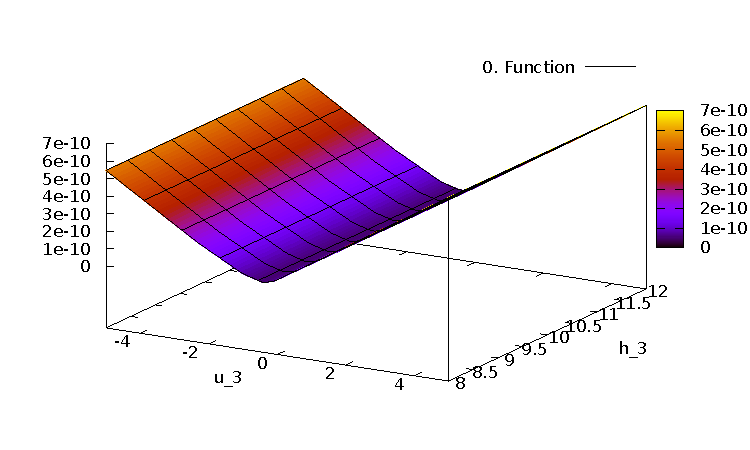
\includegraphics[scale=\zoomfactor]{{{3_punkte_2_impuls_verringert/0.0_10.0_0.0_10.0_-1.0_10.0_0.0_10.0_x_y_0.0_10.0f0}}}  
%    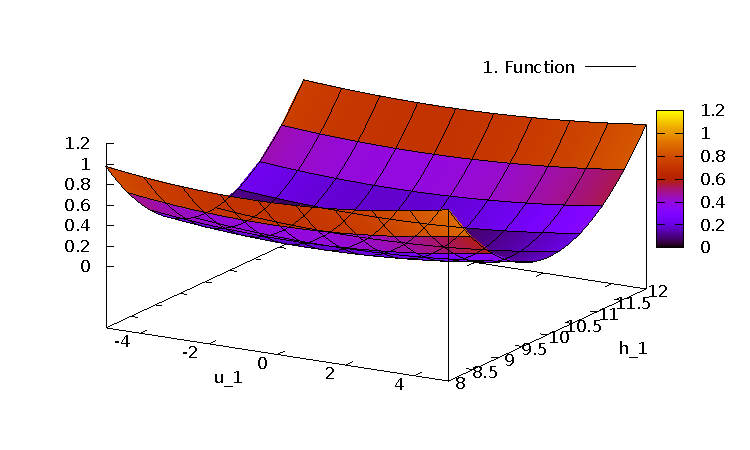
\includegraphics[scale=\zoomfactor]{{{3_punkte_2_impuls_verringert/x_y_0.0_10.0_-1.0_10.0_0.0_10.0_0.0_10.0_0.0_10.0f1}}}  
  }

  \subfigure[Height for points $p_2^L$ and $p_2^R$. Slight difference in scale.] {
    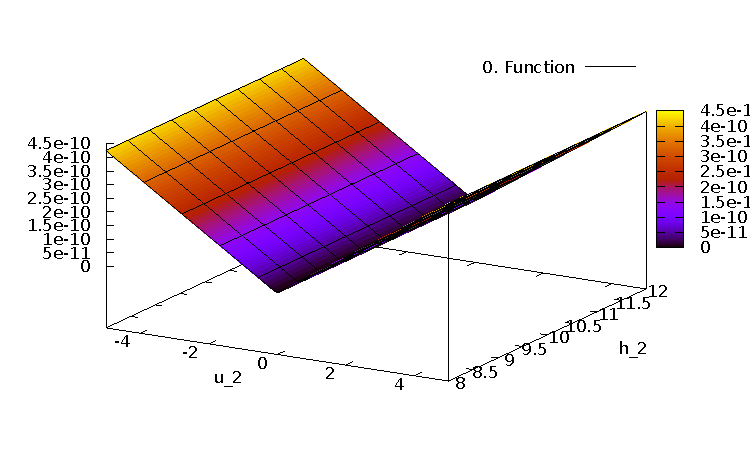
\includegraphics[scale=\zoomfactor]{{{3_punkte_2_impuls_verringert/0.0_10.0_0.0_10.0_x_y_0.0_10.0_0.0_10.0_0.0_10.0f0}}}  
    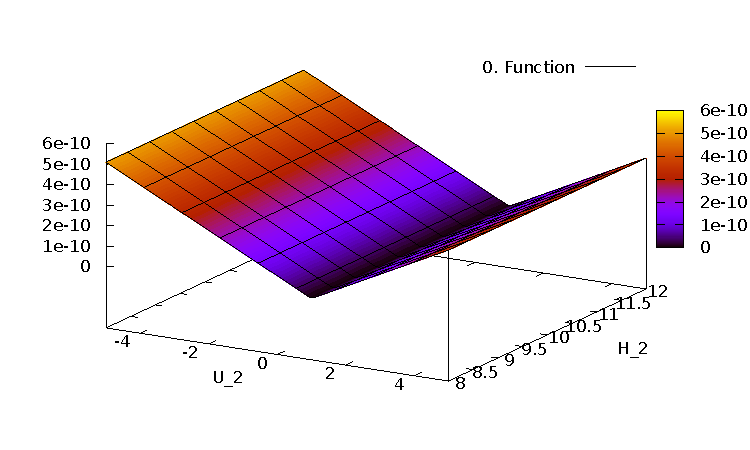
\includegraphics[scale=\zoomfactor]{{{3_punkte_2_impuls_verringert/0.0_10.0_0.0_10.0_-1.0_10.0_x_y_0.0_10.0_0.0_10.0f0}}}  
%    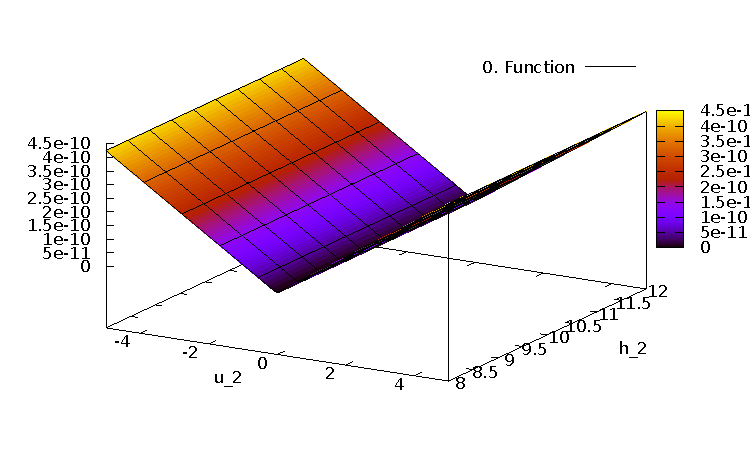
\includegraphics[scale=\zoomfactor]{{{3_punkte_2_impuls_verringert/0.0_10.0_0.0_10.0_x_y_0.0_10.0_0.0_10.0_0.0_10.0f0}}}  
%    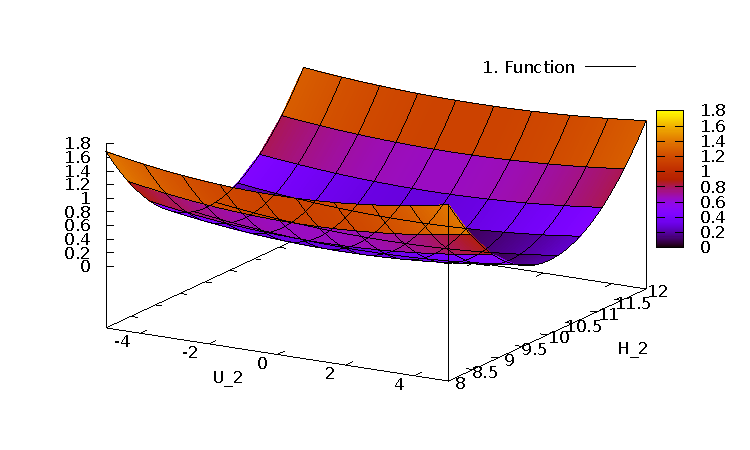
\includegraphics[scale=\zoomfactor]{{{3_punkte_2_impuls_verringert/0.0_10.0_0.0_10.0_0.0_10.0_x_y_0.0_10.0_0.0_10.0f1}}}  
  }

  \subfigure[Impulse for points $p_1^L$ (same for $p_3^L$) and $p_2^L$.] {
    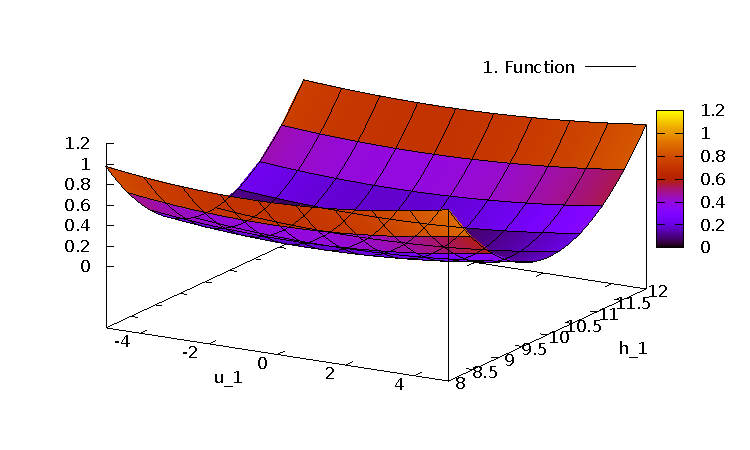
\includegraphics[scale=\zoomfactor]{{{3_punkte_2_impuls_verringert/x_y_0.0_10.0_-1.0_10.0_0.0_10.0_0.0_10.0_0.0_10.0f1}}}  
    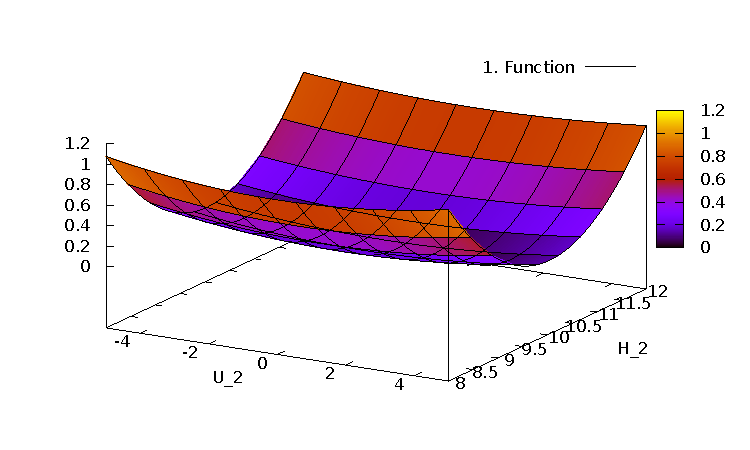
\includegraphics[scale=\zoomfactor]{{{3_punkte_2_impuls_verringert/0.0_10.0_0.0_10.0_-1.0_10.0_x_y_0.0_10.0_0.0_10.0f1}}}  
%    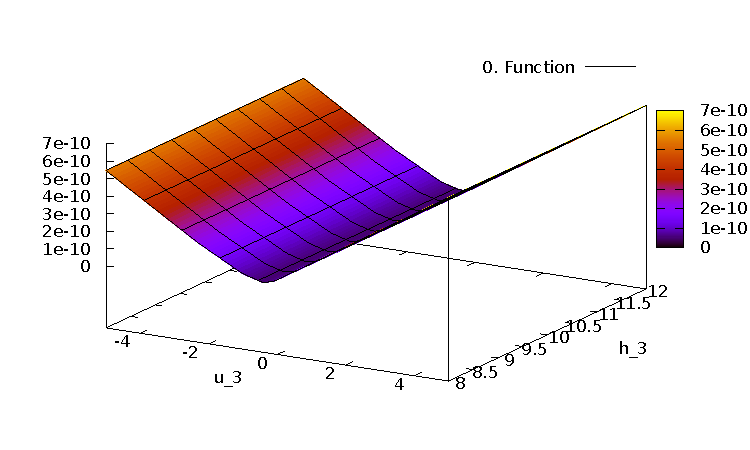
\includegraphics[scale=\zoomfactor]{{{3_punkte_2_impuls_verringert/0.0_10.0_0.0_10.0_-1.0_10.0_0.0_10.0_x_y_0.0_10.0f0}}}  
%    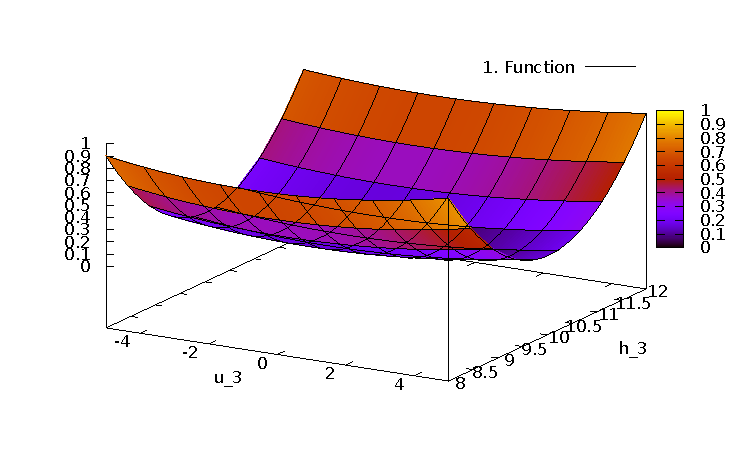
\includegraphics[scale=\zoomfactor]{{{3_punkte_2_impuls_verringert/0.0_10.0_0.0_10.0_-1.0_10.0_0.0_10.0_x_y_0.0_10.0f1}}}  
  }

%  \subfigure[Height and impulse for point $P_1$] {
%    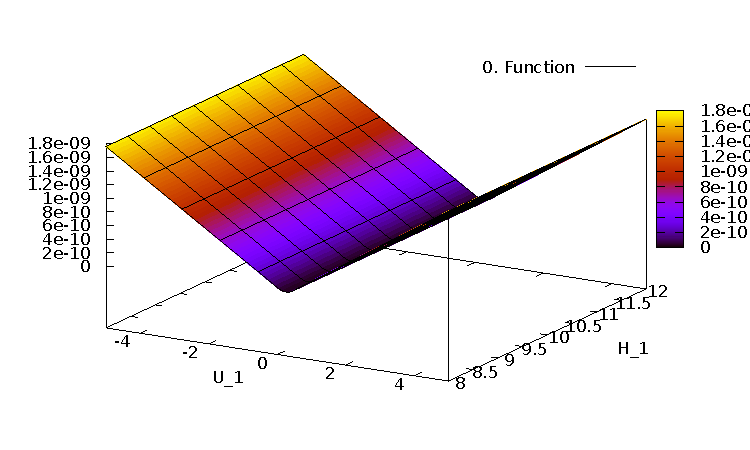
\includegraphics[scale=\zoomfactor]{{{3_punkte_2_impuls_verringert/0.0_10.0_x_y_-1.0_10.0_0.0_10.0_0.0_10.0_0.0_10.0f0}}}  
%    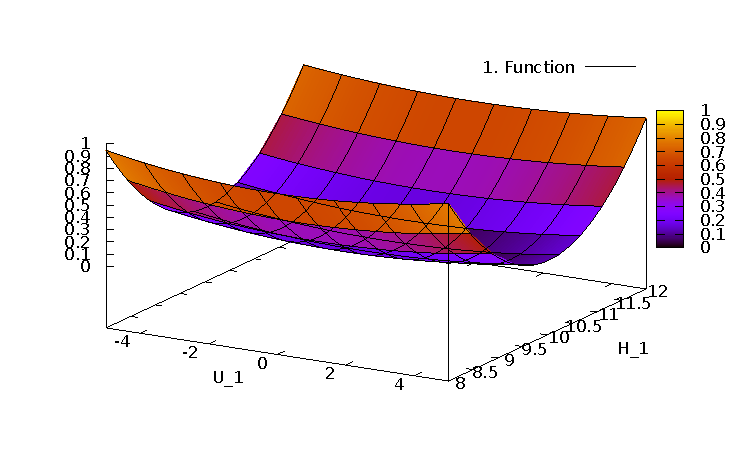
\includegraphics[scale=\zoomfactor]{{{3_punkte_2_impuls_verringert/0.0_10.0_x_y_-1.0_10.0_0.0_10.0_0.0_10.0_0.0_10.0f1}}}  
%  }

%  \subfigure[Height and impulse for point $P_2$] {
%    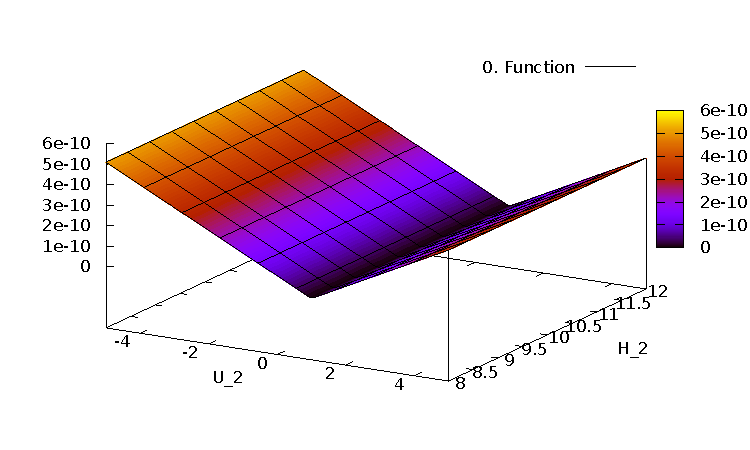
\includegraphics[scale=\zoomfactor]{{{3_punkte_2_impuls_verringert/0.0_10.0_0.0_10.0_-1.0_10.0_x_y_0.0_10.0_0.0_10.0f0}}}  
%    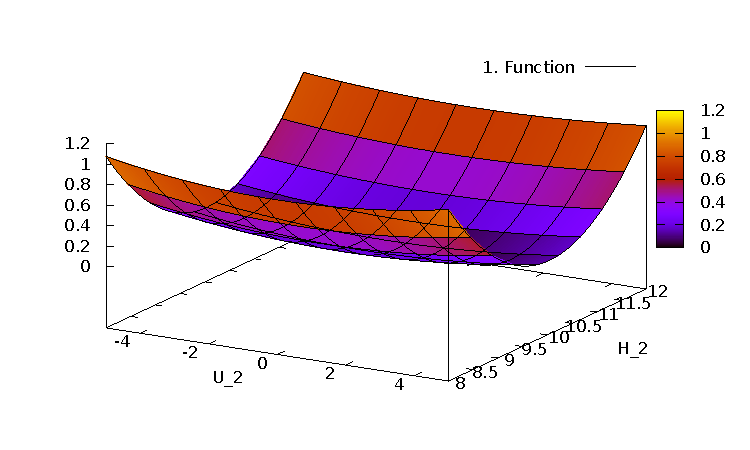
\includegraphics[scale=\zoomfactor]{{{3_punkte_2_impuls_verringert/0.0_10.0_0.0_10.0_-1.0_10.0_x_y_0.0_10.0_0.0_10.0f1}}}  
%  }

%  \subfigure[Height and impulse for point $P_3$] {
%    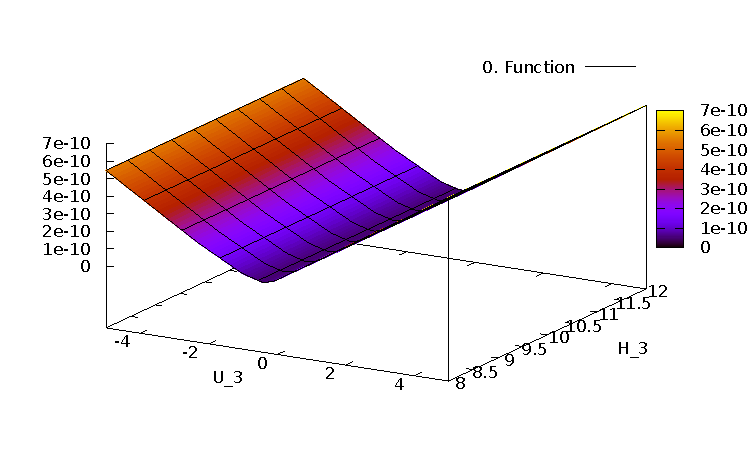
\includegraphics[scale=\zoomfactor]{{{3_punkte_2_impuls_verringert/0.0_10.0_0.0_10.0_-1.0_10.0_0.0_10.0_0.0_10.0_x_yf0}}}  
%    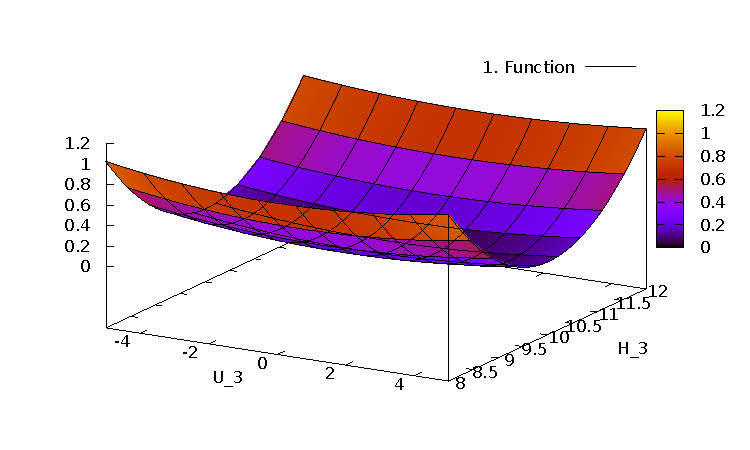
\includegraphics[scale=\zoomfactor]{{{3_punkte_2_impuls_verringert/0.0_10.0_0.0_10.0_-1.0_10.0_0.0_10.0_0.0_10.0_x_yf1}}}  
%  }
  \caption{Three points for each triangle. All points except $p_2^L$ have height 10, impulse 0. Point $p_2^L$ is set to $(10,-1)$. The resulting error graphs look the same on both triangles for each point ($p_i^L$ and $p_i^R$), with only slight variation in $p_2^L$, due to that point's impulse being different to $p_2^R$'s. The shape between the points is the same, only the scale differs.}
  \label{fig:three-points-u2-}
\end{figure}

%%% Local Variables:
%%% TeX-master: "../results.tex"
%%% End:
